\chapter[Introduction]{Introduction}\label{chap_intro}

\section{Motivation}
\label{Sec:Motivation}

Recent works \cite{Ghanta022019, Crankshaw2017, Polyzotis2018}, highlight some of the challenges encountered in spatio-temporal predictive serving systems. In such systems, values of variables whose behavior vary in space-time are inferred by predictive models built over regions of the spatio-temporal domain. In this context, we are interested in the problem arising in the presence of multiple competing predictive models, i.e. models that predict the same variable but built independently over potentially different regions of the domain. This may be the case in large companies in which autonomously developed models about the same phenomenon (a.k.a. competing models) are deployed and used to answer predictive queries. 
%In this context, the training and validation processes used in building competing models may consider \fab{improve}different fragments of the modeled phenomenon domain leading to a variation on their predictive accuracy.

A predictive serving system enables users to express predictive queries that specify: a spatio-temporal region; a predictive variable and a evaluation metric. The outcome of a predictive query present the values of the predictive variable on the specified region computed by predictive models that maximize the evaluation metric. 

Identifying the predictive models to be used by the system to answer the predictive query is, however, a hard problem. This is due to the fact that competing predictive models present varying predictive behavior through regions of the domain. This maybe due to learners intrinsic learning capabilities and/or variations on spatio-temporal regions used during the construction of independently built models. In this context, our goal is to define a procedure that selects a set of models that computes the query answer and maximizes the evaluation metric, see Figure \ref{Fig:MotiPoster}. 

\begin{figure}[h]
	\centering
	
\includegraphics[scale=0.3]{../Figures/ModelManagementPS-VersionCompleta}
	\caption{Predictive Serving System Models.}
	\label{Fig:MotiPoster}
	%	\Description{ML Model Lifecycle.}
\end{figure}

Our approach objective is quantify the predictive quality for auto-regressive models using a shape-based characterization of the domain. 
%about the predictive variable domain data distribution. 
In particular, we compute the data distribution on regions of the domain where the models have been trained and compare them against those within the query spatio-temporal region. The intuition is that models behavior in query regions with similar data distribution as the ones used to train the model, shall follow the one observed during training. Conversely, in spatio-temporal regions specified by the query and that have not been used for training the model would exhibit an error computed as a function of the distance between the query non seen data region and the model building data region.

\subsection{Problem Statement}
\label{Sec:ProblemStatement}

Given a phenomenon with a spatio-temporal domain, represented by univariate time series, where independent predictive models have been trained, select a model or a composition of models to answer a spatio--temporal predictive query that maximizes an evaluation metric.

\section{Objective and Contribution}
\label{Sec:ObjectiveContribution}

(TODO) Our approach aims to quantify the predictive quality of models, by characterizing patterns within the predictive variable domain data. In particular, we identify some patterns on domain regions where the models have been trained, and compare them against patterns within the query spatio-temporal region. Our intuition is that, if a query region has similar data patterns as the regions used to train the model, then the behavior of the model on the query region should follow the one observed during training.
Conversely, in spatio-temporal regions specified by the query, that have not been used for training, the model would exhibit an error computed as a function of the distance between the query non seen data region and the model building data region.

A collection of time series can exhibit various dependency relationships between the individual time series that can be leveraged in forecasting. These include: (1) local co-variate relationships (e.g. the price and demand for a product, which tend to be (negatively) correlated), (2) indirect relationships through shared latent causes (e.g. demand for multiple products increasing because an advertising campaign is driving traffic to the site), (3) subtle dependencies through smoothness, temporal dynamics, and noise characteristics of time series that are measurements of similar underlying phenomena (e.g. product sales time series tend to be similar to each other, but different from energy consumption time series).The data in practical forecasting problems typically has all of these forms of dependencies. Making use of this data from related time series allows more complex and potentially more accurate models to be fitted without overfitting.

\section{Problem Formalization}
\label{Sec:ProblemFormalization}

Let $\mathcal{D} = \{(\mathcal{S}, x, y): \,\, \mathcal{S} = \{s_{1}, s_{2}, \ldots, s_{t}\}$ is a univariate time--series, and $(x,y) \in \mathbb{R}^{2}\}$, represents a spatio-temporal domain. Denote by $\mathcal{G} = \{g: \mathbf{S} \to \mathbf{S}$ such that $g(\mathcal{S}) = \mathcal{S}\}$, the set of temporal predictive models for $\mathbf{S} \subseteq \mathcal{D}$. Each predictive model $g\in \mathcal{G}$ is denoted as follows:
\begin{equation}
\label{eq:ModelDefinition}
g = \langle \mathbf{S}, A, \mathbf{p}, E, \varSigma \rangle,
\end{equation}
where:
\begin{itemize}[noitemsep,nolistsep]	
	\item $\mathbf{S}$: input dataset included in the spatio--temporal domain $\mathcal{D}$,
	\item $A$: learner or hypothesis set,
	\item $\mathbf{p}$: model parameters (number of time-units to obtain the generalization error ($t_{p}$), number of time-units to forecast ($t_{f}$)),
	\item $E$: generalization error,
	\item $\varSigma$: implementation/execution quality metrics.
\end{itemize}

%TODO Extend the existence for several competing models.
\noindent In this context, given a predictive spatio--temporal query $Q$ denoted as:
\begin{equation} \label{eq:predictivequery}
Q = \langle R, t_{p}, t_{f}, Q_{m} \rangle,
\end{equation}
where:
\begin{itemize}[noitemsep,nolistsep]	
	\item $R$: represents the size/shape/type of interest region,
	\item $t_{p}$: $\{s_{t-t_p}, s_{t-t_{p}+1}\ldots, s_{t}\}$ number of steps used for  prediction,
	\item $t_{f}$: $\{s_{t+1}, \ldots, s_{t+t_f}\}$ number of steps to predict ($n\geq 1$),
	\item $Q_{m}$: represents users qualitative measurements to evaluate the predictive output.
\end{itemize}

We formally define our problem: Let the spatio-temporal domain characterization $\mathcal{D} = \bigcup_{i=1}^{n} \mathbf{S_i}$ and $\mathcal{G}$ the set of temporal models for a single element of $\mathbf{S_i}$ that accounts for the generalization error bounds for the elements in $\mathbf{S_i}$. Given $Q = \langle R, t_{p}, t_{f}, Q_{m} \rangle$:

\begin{equation}
\forall \mathcal{S} \in R: \exists g \in \mathcal{G'} \,\,\textrm{such that} \,\, \argminA_{g\in\mathcal{G'}} E_{g}(R).
\end{equation}

%TODO Change the argmin 
\noindent In Figure \ref{fig:time-series}, we show the elements involved in the formalization of our problem:
\begin{figure}[htb]
	%\begin{minipage}[b]{0.8\textwidth}
	\centering
	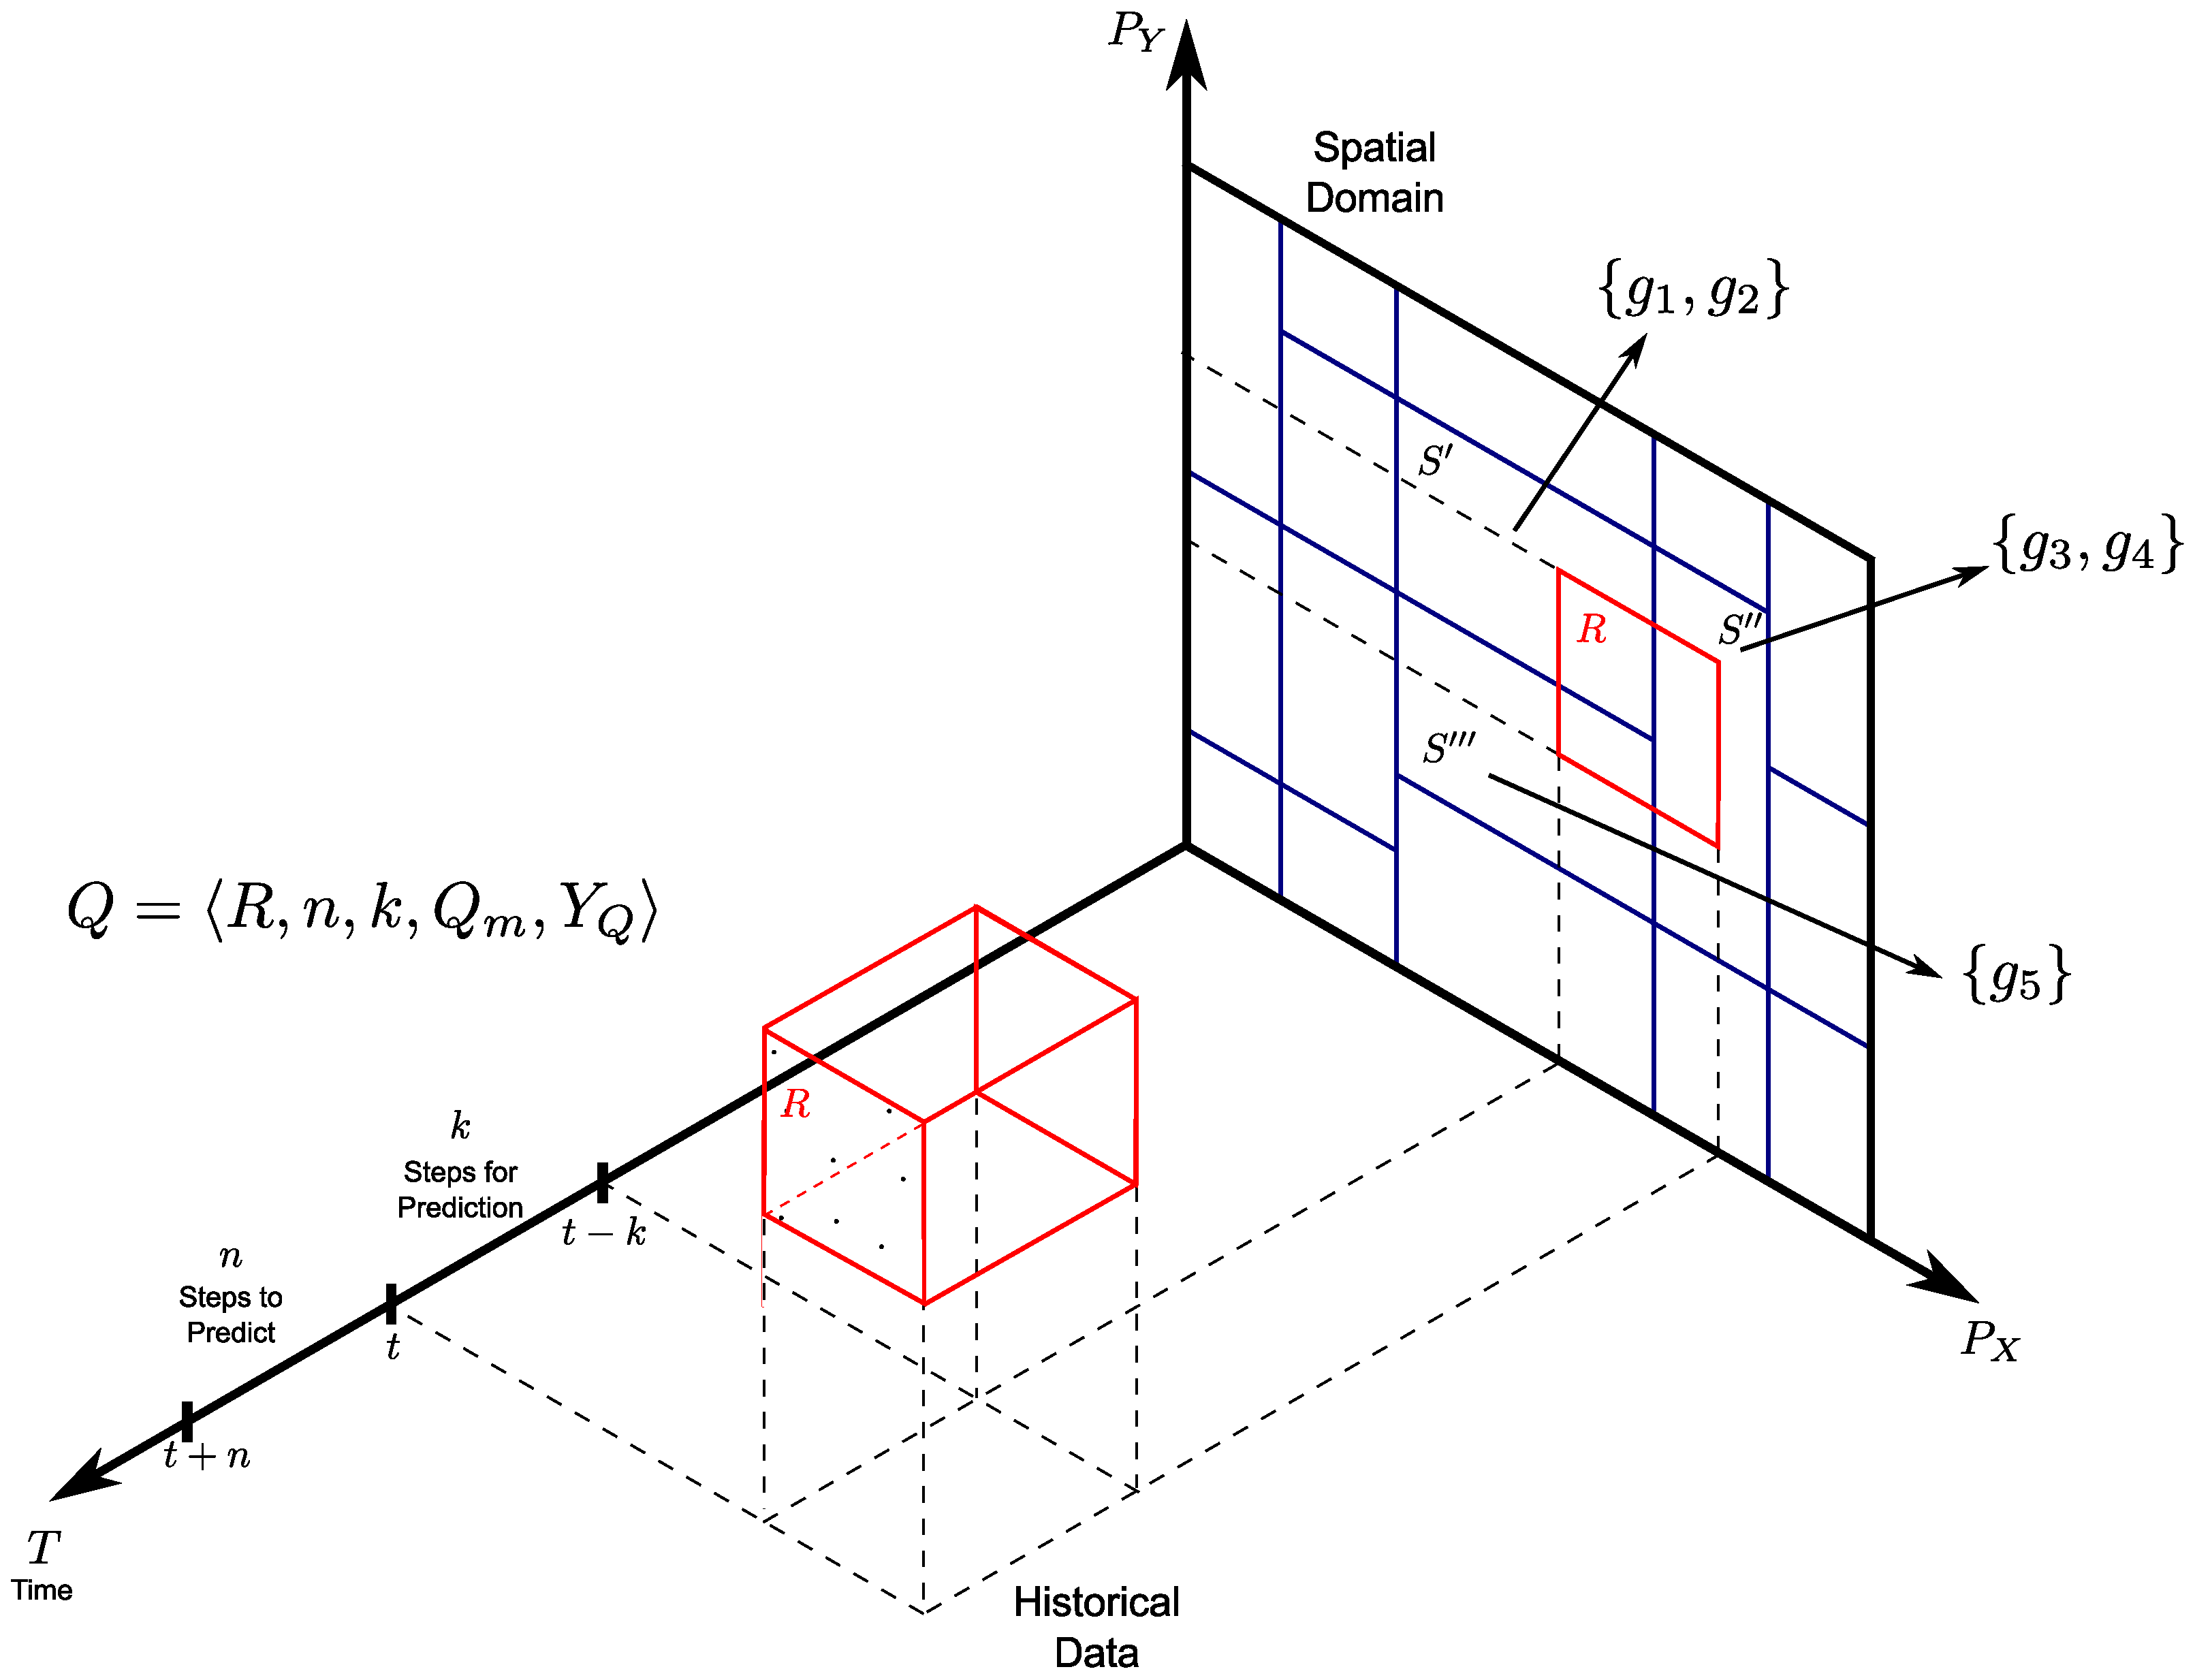
\includegraphics[scale=0.25]{../Figures/RepresentationTimeSeries}
	\caption{Predictive Spatio--Temporal Queries.}
	\label{fig:time-series}
	%\end{minipage}
\end{figure}


\section{Thesis Outline}
\label{Sec:ThesisOutline}

The structure of the remainder of this thesis is outlined for reference.

\begin{description}
\item[Chapter 2.] \textbf{[Theoretical Foundations.]}
\item[Chapter 3.] \textbf{[Related Works.]}
\item[Chapter 4.] \textbf{[Methodology.]} 
\item[Chapter 5.] \textbf{[Implementation and Experimental Results.]}
\item[Chapter 6.] \textbf{[Conclusions and Future Works.]}
\end{description}

% TODO Include in the Introduction
% A hypothesis we want to highlight is that it should be preferable to use a partitioning technique that considers grouping domain elements based on the similarity of their temporal evolution, rather than creating groups just according to a regular division of the domain geometry. To verify this, we compare the intra-cluster sum of both partitioning techniques for several values of $k$.